\documentclass[a4paper]{article}
\usepackage[utf8]{inputenc}
\usepackage{fullpage}
\usepackage{amsmath,amssymb}
\usepackage[colorlinks,linkcolor=blue]{hyperref} % use colored text in stead of ugly boxes
\usepackage[toc]{multitoc} % Nice two-column TOC

\usepackage{graphicx}
\usepackage{tabto}

\usepackage{pdfpages}
%~ TikZ is not in use in this document
%~ \usepackage{pgf}
%~ \usepackage{tikz}
%~ \usepackage{pictures/tikz-uml}

% new line after paragraph title.
\makeatletter
\renewcommand\paragraph{\@startsection{paragraph}{4}{\z@}%
  {-3.25ex\@plus -1ex \@minus -.2ex}%
  {1.5ex \@plus .2ex}%
  {\normalfont\normalsize\bfseries}}
\makeatother


\title{Programming Life - Final report}

\author{Group E:\\
Felix Akkermans \\
Niels Doekemeijer \\
Thomas van Helden \\
Albert ten Napel \\
Jan Pieter Waagmeester}

\begin{document}
\maketitle

\vfill

\small{\tableofcontents}
\pagebreak

\section*{Abstract}
This document concludes the whole \textit{Contextproject} and especially the development of our product: Zelula. This piece of software provides synthetic biologists with a visual tool to design, simulate and validate biological logic circuits.

The project was roughly devided in two parts: the design stage and the implementation stage. Both were roughly of equal length.

todo fix more.

\section{Introduction}


%images used:
\pgfdeclareimage[width=0.45\textwidth]{gui-final}{pictures/gui_final1.png}
\pgfdeclareimage[width=0.45\textwidth]{gui-input-csv}{pictures/define-inputs-csv.png}
\pgfdeclareimage[width=0.45\textwidth]{gui-input-editor}{pictures/define-inputs-editor.png}
%~ \pgfdeclareimage[width=0.45\textwidth]{gui-final}{pictures/gui_final_spitscreen.png}

\newcommand{\screenshotScale}{1.4}



\section{Description of Zelula}
Zelula is a modelling and simulation package which enables users to simulate the protein \textit{logic} in a cell. With a provided set of BioBricks representing AND and NOT gates, the user is able to design interactions between the different BioBricks. The resulting circuits can be simulated, the results will be presented as a concentration/time graph.


\subsection{Circuit editor}
\begin{figure}[h!]
\centering\begin{tikzpicture}[scale=\screenshotScale]
	\pgftext[left, base]{\pgfuseimage{gui-final}}
	\draw [draw=red,very thick] (0, 2.4) -- (0, 3.7) -- (7.15, 3.7) -- (7.15,0.14) -- (1.5,0.14) -- (1.5, 2.4) -- (0,2.4);
\end{tikzpicture}
\caption{GUI mainscreen; highlighted is the workspace with the regular (draggable) gates.}
\end{figure}

\noindent Zelula enables the user to intuitively construct circuits from the basic available building blocks (see figure 1 for the mainscreen). Gates can be dragged from the sidebar to arbitrary positions in the working area. Connections between the gates can easily be dragged from and to the \textit{input} and \textit{output} connectors and the endpoints on gates. 

When a connection is made, no protein is selected for it by default. The user may select which protein to use. Visual feedback on protein assignment is provided through the colors of the connections.

The interface prevents the user to make some simple mistakes. For example, it's impossible to connect two inputs. If the user connects one output to two inputs, the interface makes sure the protein on those connections is the same.

Even the position of the circuits' input and output connectors can be freely chosen by dragging them using the text as an handle.

Removing gates and connection is a matter of double clicking on them.

\newpage
\subsection{Compound library}
\begin{figure}[h!]
\centering\begin{tikzpicture}[scale=\screenshotScale]
	\pgftext[left, base]{\pgfuseimage{gui-final}}
	\draw [draw=red,very thick] (0,0.14) rectangle (1.5, 2.5);
\end{tikzpicture}
\caption{GUI mainscreen; highlighted is the box with the (draggable) compound gates.}
\end{figure}

\noindent Every circuit can be saved as a compound gate, which means it can easily be reused in later circuits. The saved compound gates are presented to the user in the sidebar, below of the basic gates (figure 2). When a user drags a compound gate to the working area, it will expand to the original arrangement of gates, with the inner connections in place. The only thing left for the user is connecting it to the rest of its circuit.

\subsection{Validation}
When a user is satisfied with his work, he can validate the circuit. Different errors like unassigned proteins or inclomplete connections will be reported. The user will see the error message below the circuit, providing excellent overview to both the circuit and the errors to solve the problem.

\subsection{Simulation}
A valid circuit can be simulated. In order to simulate a circuit, the input must be defined as a function of time. Zelula provides two ways to accomplish this. Firstly, in an input editor the level for each input can be defined as a function of time in a visual way, secondly, a CSV text can be provided describing the transitions as a function of time.

\paragraph{Input editor}
\begin{figure}[h!]
\centering\begin{tikzpicture}[scale=\screenshotScale]
	\pgftext[left, base]{\pgfuseimage{gui-input-editor}}
\end{tikzpicture}
\caption{Dialog for defining input values per protein in client.}
\end{figure}

\noindent The input editor (figure 3) enables the user to define each input signal in a visual way. Each tick represents a number of seconds in the simulation. The user can select this number of seconds, and also the number of ticks available.

When a user clicks on a tick, it is toggled. The user may also select ranges by clicking on a certain tick an dragging the mouse to another tick while holding the mouse button.

\newpage
\paragraph{CSV input}
\begin{figure}[h!]
\centering\begin{tikzpicture}[scale=\screenshotScale]
	\pgftext[left, base]{\pgfuseimage{gui-input-csv}}
\end{tikzpicture}
\caption{Dialog for defining input values in client by CSV.}
\end{figure}

\noindent The input may also be defined by a simple CSV format (figure 4), as defined by the SA.

\subsection{Exporting}
The work done in Zelula can be shared in two different ways: the user can export the circuit to a SBML file, a common format uses in syntetic Biology.

Secondly, the visualistion of the graphs can be exported to a number of different image formats.

\subsection{Server}
The server operates in the background, serving the files needed for the GUI, providing file storage and simulation services. The user does not interact with it in a direct way.

The servlets depends on Tomcat and might be distribugted as a \verb|.war| archive. 


\section{Design and implementation process}
The first half of the project was focused on design, while the second part was all about implementation. In this chapter we will reflect on the consistency between design and implementation. We will clarify what was implemented according to the documents and what was changed or perhaps not implemented.

In the Test \& Implementation plan\footnote{linkie linkie} we set up a list of requirements according to the MoSCoW model. What follows is a copy of this list with comments on how (and if) it is implemented, but first we will give a quick comparison of the intended and eventual GUI design.

\subsection{Client GUI}
In our RAD document\footnote{linkie linkie} we gave a few simple sketches of what we had in mind for the user interface of the client.

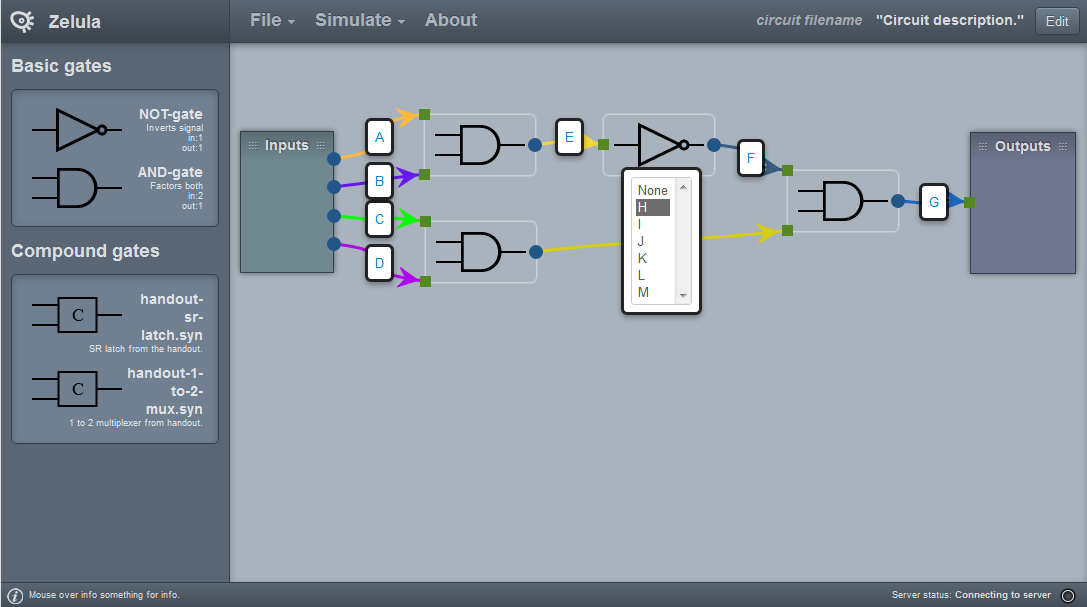
\includegraphics[width=15cm]{pictures/gui_final1.png}

\subsection{Must-Haves}
\begin{description}
\item[1. Connection] \textit{Client and server must be able to communicate. If there is no connection, the user should be notified.}\\
This is an explanation.

\item[2. Available gates] \textit{The application must be able to present a list of available gates to the user. These gates can be used to model the circuit.}\\
This is an explanation.

\item[3. Design circuit] \textit{The user must be able to design a circuit by specifying gates (using a drag-and-drop) and the relations between these gates.}
	\begin{itemize}
	\item \textbf{3.1} \textit{The application must be able to visualize a gate using a simplified image. This image should relate to the function of the gate. For example, for the AND gate, it is logical to use the distinctive AND symbol normally used in circuit design.}\\
	This is an explanation.

	\item \textbf{3.2} \textit{The user must be able to drag and drop gates from the list into the working area.}\\
	This is an explanation.

	\item \textbf{3.3} \textit{The user must be able freely to move the gate around in the working area, but gates will snap to grid points on the working area.}\\
	This is an explanation.

	\item \textbf{3.4} \textit{The user must be able to draw connections between the gates in the form of wires.}\\
	This is an explanation.

	\item \textbf{3.5} \textit{The user must be able to draw input and output wires for the circuit, to explicitly state which proteins will be used as input.}\\
	This is an explanation.

	\end{itemize}
\item[4. Available proteins] \textit{The application must be able to present the user with an overview of available proteins to assign to signals (visualized by the wires).}\\
This is an explanation.

\item[5. Protein specification] \textit{The user must be able to specify which protein is used for a certain signal.}\\
This is an explanation.

\item[6. Export circuit] \textit{The application must to able to save a circuit to a .syn file.}\\
This is an explanation.

\item[7. Import circuit] \textit{The application must be able to load an exported circuit from a .syn file.}\\
This is an explanation.

\item[8. Input values specification] \textit{The user must be able to specify the input values used for the simulation of the circuit.}\\
This is an explanation.

\item[9. Circuit validation] \textit{The user must to be able validate his circuit in the application and get feedback over where there are conflicts.}\\
This is an explanation.

\item[10. Circuit simulation] \textit{The application must be able to simulate a valid circuit and present the output values to the user.}\\
This is an explanation.
\end{description}

\subsection{Should-Haves}
\begin{description}
\item[11. Re-use circuits] \textit{The application can import pre-defined circuits as extra gates. This is not a necessity, but would be a great addition to the program (and will ease building circuits). Among others, protein specification, importing and exporting will be more difficult to implement.}\\
This is an explanation.
\end{description}


\section{Key problems and solutions - highlights}

During this project we have encountered some problems. In this section we will have a look at some of the highlights of these problems and how we fixed them.

Our program was developed test driven. This makes for very neat code, but it also comes with some problems. We mainly encountered problems with QUnit, a JQeury testing framework similar to Java's JUnit. Although the testing was done properly, the feedback on the results was not very helpful. Eventually we managed to tackle this problem with some extra manual testing.

A common issue using server-client structure is the actual connection between the two. In the beginning we had some trouble with this but this was mainly caused by out of sync code and trouble with Apache Tomcat. We decided on a standard version of Tomcat and wrote a setup page on the wiki. Afterwards, the problem was solved.

Another problem client side was the dragging and dropping of gates and connecting them with wires. We had anticipated this as being tough and found a solution in jsPlumb, a solution with its downsides. The framework jsPlumb makes it easy to create connectors and draw wires between gates, but it didn't fully meet our needs so we had to customize it, leading to quite some hours of extra work. (NIELS MORE EXPLANATION)

At one point, we figured we wanted to select our proteins from dropdown menus on our wires. Regular dropdown menus from Javascript are not an issues, however combining this with jsPlumb and bootstrap proved to be a little more difficult. This took more time than we had anticipated but was eventually solved after trying several options.

Throughout this project we worked with Git and GitHub to share our code. We also used the ticket mechanism of GitHub to keep track of what had to be done. Git is exceptionally good at merging code but cannot always prevent conflicts. If there is too little communication between two people who are working on the same code, merging can become difficult. However, with some reverts and recommitting these problems were resolved.

Towards the end of our project, we did some major restructuring. We shifted some functions around, changed some names and did some more testing and commenting. We did this based on the feedback we got from the SIG evaluation. The biggest changes were made on the client side.

Our program is not only to model circuits but also to calculate and display the outcome. We displayed the outcome in a graph, but this showed some weird results. It turned out that the solver for our circuits had some issues (ALBERT EXPLAIN HOW IT WAS SOLVED).

\section{Reflection on the teamwork}

\section{Individual reflection on the project} %max 1 A4 per teammember
\subsection{Felix Akkermans}
\subsection{Niels Doekemeijer}
\subsection{Thomas van Helden}
\subsection{Albert ten Napel}
\subsection{Jan Pieter Waagmeester}

\section{Lightweight SCRUM Plans}
The following pages will include the relevent parts of our lightweight scrumplans for each iteration. The colored links and numbers with a hashtag refer to GitHub issues on \url{https://github.com/FelixAkk/synthbio/issues}. For each iteration, a milestone is available providing a nice overview of the issues for each iteration.

\includepdf[
	landscape, frame, nup=1x2, pages=2-3,
	addtotoc={2 , subsection , 1 , Scrumplan 1 , scrum-1}
]{../scrumplan-1/scrumplan-1.pdf}

\includepdf[
	landscape, frame, nup=1x2, pages=2-3,
	addtotoc={2 , subsection , 1 , Scrumplan 2 , scrum-2}
]{../scrumplan-2/scrumplan-2.pdf}

\includepdf[
	landscape, frame, nup=1x2, pages=2-3,
	addtotoc={2 , subsection , 1 , Scrumplan 3 , scrum-3}
]{../scrumplan-3/scrumplan-3.pdf}

\includepdf[
	landscape, frame, nup=1x2, pages=2-3,
	addtotoc={2 , subsection , 1 , Scrumplan 4 , scrum-4}
]{../scrumplan-4/scrumplan-4.pdf}


\end{document}
